\documentclass[12pt,-letter paper]{article}
\usepackage{siunitx}
\usepackage{setspace}
\usepackage{gensymb}
\usepackage{xcolor}
\usepackage{caption}
%\usepackage{subcaption}
\doublespacing
\singlespacing
\usepackage[none]{hyphenat}
\usepackage{amssymb}
\usepackage{relsize}
\usepackage[cmex10]{amsmath}
\usepackage{mathtools}
\usepackage{amsmath}
\usepackage{commath}
\usepackage{amsthm}
\interdisplaylinepenalty=2500
%\savesymbol{iint}
\usepackage{txfonts}
%\restoresymbol{TXF}{iint}
\usepackage{wasysym}
\usepackage{amsthm}
\usepackage{mathrsfs}
\usepackage{txfonts}
\let\vec\mathbf{}
\usepackage{stfloats}
\usepackage{float}
\usepackage{cite}
\usepackage{cases}
\usepackage{subfig}
%\usepackage{xtab}
\usepackage{longtable}
\usepackage{multirow}
%\usepackage{algorithm}
\usepackage{amssymb}
%\usepackage{algpseudocode}
\usepackage{enumitem}
\usepackage{mathtools}
%\usepackage{eenrc}
%\usepackage[framemethod=tikz]{mdframed}
\usepackage{listings}
%\usepackage{listings}
\usepackage[latin1]{inputenc}
%%\usepackage{color}{   
%%\usepackage{lscape}
\usepackage{textcomp}
\usepackage{titling}
\usepackage{hyperref}
%\usepackage{fulbigskip}   
\usepackage{tikz}
\usepackage{graphicx}
\lstset{
  frame=single,
  breaklines=true
}
\let\vec\mathbf{}
\usepackage{enumitem}
\usepackage{graphicx}
\usepackage{siunitx}
\let\vec\mathbf{}
\usepackage{enumitem}
\usepackage{graphicx}
\usepackage{enumitem}
\usepackage{tfrupee}
\usepackage{amsmath}
\usepackage{amssymb}
\usepackage{mwe} % for blindtext and example-image-a in example
\usepackage{wrapfig}
\graphicspath{{figs/}}
\providecommand{\mydet}[1]{\ensuremath{\begin{vmatrix}#1\end{vmatrix}}}
\providecommand{\myvec}[1]{\ensuremath{\begin{bmatrix}#1\end{bmatrix}}}
\providecommand{\cbrak}[1]{\ensuremath{\left\{#1\right\}}}
\providecommand{\brak}[1]{\ensuremath{\left(#1\right)}i}
\begin{document}
\begin{enumerate}
	\item Show that \begin{align}(a-b)^2,(a^2+b^2) and (a+b)^2\end{align} are in $AP$
		\item In Fig. 1, $DE|| AC$ and $DC|| AP$. Prove that \begin{align}\frac{BE}{EC} =
		\frac{BC}{CP}\end{align}.
		\begin{figure}[H]
		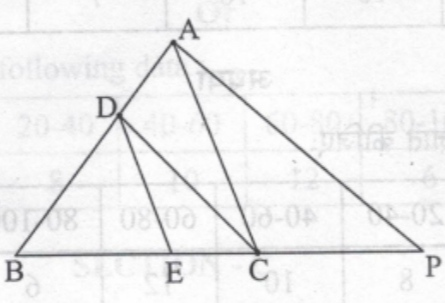
\includegraphics[width=\columnwidth]{./imagecharan1.jpg}
		\label{fig:fig1}
		\caption{figure}
		\end{figure}


	\item In Fig.2, two tangents $TP$ and $TQ$ are drawn to a circle with centre $O$ from an external point. prove that \begin{align}\angle PTQ = 2\angle OPQ\end{align}
		\begin{figure}[H]                                                                         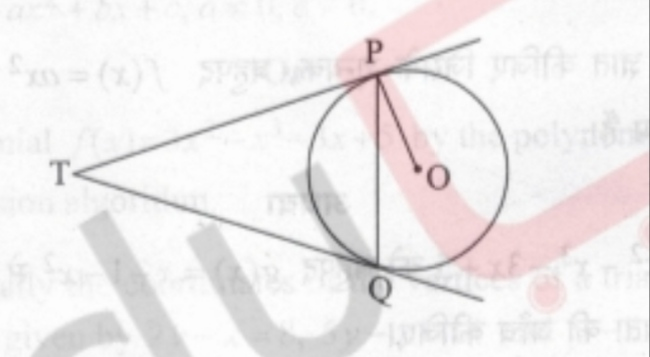
\includegraphics[width=\columnwidth]{./imagecharan2.jpg}                          \label{fig:fig1}                                                                  \caption{figure}                                                          \end{figure}
		\item The rod $AC$ of a $TV$ disc antenna is fixed at the right angles to the wall $AB$ and a rod $CD$ is supporting the disc as shown in $fig.3$. IF $	AC=1.5$ long and $CD=3m$, find \begin{align}\textit{(i)}\tan\theta \textit{(ii)}\sec\theta\end{align}.
	\begin{figure}[H] 
		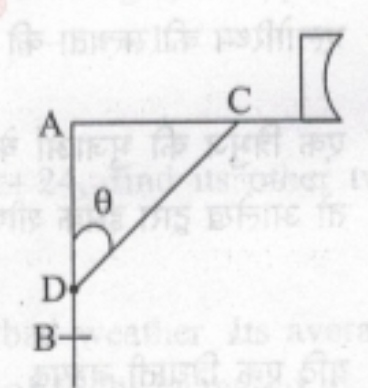
\includegraphics[width=\columnwidth]{./imagecharan3.jpg} 
		\label{fig:fig1}
		\caption{}
	\end{figure}


\item A piece of wire $22cm$ long is bent into the form of an arc of a circle subtending an angle of $60^\circ$ as it's centre.Find the radius of the circle \begin{align}\myvec{use\pi=\frac{22}{7}}\end{align}
	\item If Anumber x is choosen at random from the numbers \begin{align}-3,-2,-1,0,1,2,3\end{align}. what is probability that \begin{align}x^2 \leq4\end{align}
		\item Find quadratic polynomial whose zeroes are reciprocal of the zeroes of the polynomial \begin{align}f(x)=ax^2+bx+c, a\neq 0,c\neq 0\end{align}
			\item Divide the polynomial \begin{align}f(x)=3x^2-x^3-3x+5\end{align} by the polynomial \begin{align}g(x)=x-1-x^2\end{align} and verify the division algorithm
		 
				\item Determine graphically the coordinates of the vertices of a triangle , the equations of whose sides are given by \begin{align}2y-x=8, 5y-x=14 and y-2x=1\end{align}
					\item If y is a zero of the cubic polynomial \begin{align}x^3-3x^2-10x+2y\end{align}, find its other two zeroes
	\item In a flight of $600km$, an aircraft was slowed due to bad weather . Its average speed for the trip was reduced by $200km/hr$ and time of flight increased by $30 minutes$ . Find the original duration of flight 

	\item Fnd the area of a triangle PQR formed by the points \begin{align}P(-5,7),Q(-4,-5) and R(4,5)\end{align}.
		\item If the point $c(-1,2)$ divides internally the line segment joining $A(2,5)$ and $B(x,y)$ in the ratio $3:4,$ find the coordinate of $B$  
		\item If the point $c(-1,2)$ divides internally the line segment joining $A(2,5)$ an $B(x,y)$ in the ratio $3:4,$ find the coordinate of $B$  
		\item In $Fig.4$, \begin{align}\angle D=\angle E\end{align} and \begin{align}\frac{AD}{DB}=\frac{AE}{EC}\end{align},prove that $BAC$ is an isosceles triangle
\begin{figure}[H]    
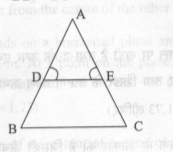
\includegraphics[width=\columnwidth]{./imagecharan4.jpg}    
\label{fig:fig1}  
\caption{triangle}  
\end{figure}

       \item In a triangle ,if square of one side is equal to the sum of the squares of the other two sides,then prove that the angle opposite to the first side is a right angle
       \item If \begin{align}\sin \theta + \cos \theta = \sqrt{3}\end{align}, then prove that \begin{align}\tan \theta + \cot \theta = 1\end{align}.
       \item $A$ cone of base radius $4cm$ is divided into two parts by drawing a place through the mid-point if its height and parallel to its base. compare the volume of the two parts 
       \item show that the square of any positive integer cannot be of the form \begin{align}(5q+2) or (5q+3)\end{align} for any integer $q$.
       \item prove that one of every  three consescutive positive integer is divisible by $3$.
       \item the sum of four consecutive numbers in $AP$ is $32$ and the ratio of the product of the first and last terms to the product of two middle terms is $7:15$. Find the numbrs 
       \item draw a line segment AB of length $7cm$. taking $A$ as centre, draw a circle of radius $3cm$ and and taking $B$ as centre, draw another circle of radius $2cm$ construct tangents tangents to each circle from the centre of the other circle.
       \item A vertical tower stands on a horizontal plane and is surrounded by a vertical flag-staff of height $6m$. At a point on the plane, the angle of elevation of the bottom and rop of the flag-staf are $30^\circ$ and $45^\circ$ respectively. find the height of the tower .(take$\sqrt{3}=1.73$)
       \item A bucket in the form of a fraction of a cone of height $30cm$ with radii of its lower and upper ends as $10cm$ and $20cm$, respectively. Find the capacity of the bucket.Also find the cost of milk which can completely fill the bucket at the rate of $Rs.40$ per litre. \begin{align}\brak {use\pi=\frac{22}{7}}\end{align}



\end{enumerate}
\end{document}
